\documentclass[a4paper,oneside,11pt]{report}
\makeatletter
\newcommand*{\rom}[1]{\expandafter\@slowromancap\romannumeral #1@}
\makeatother
\usepackage[margin=1in]{geometry}
\usepackage[doublespacing]{setspace}
\usepackage[style=authoryear,citestyle=authoryear,sorting=nyt]{biblatex}
\usepackage{graphicx}
\usepackage{wrapfig}
\usepackage{lscape}
\usepackage{rotating}
\usepackage{epstopdf}
\usepackage{listings}
\usepackage{color}

\definecolor{dkgreen}{rgb}{0,0.6,0}
\definecolor{gray}{rgb}{0.5,0.5,0.5}
\definecolor{mauve}{rgb}{0.58,0,0.82}

\lstset{frame=tb,
  language=PHP,
  aboveskip=3mm,
  belowskip=3mm,
  showstringspaces=false,
  columns=flexible,
  basicstyle={\small\ttfamily},
  numbers=none,
  numberstyle=\tiny\color{gray},
  keywordstyle=\color{blue},
  commentstyle=\color{dkgreen},
  stringstyle=\color{mauve},
  breaklines=true,
  breakatwhitespace=true
  tabsize=3
}
\addbibresource{references.bib}
\begin{document}
\title{ASCUS - Collaboration Finder}
\author{Saad Arif\\ Marticulation Number: H00011110 \\Fourth Year Dissertation - First Deliverable \\ Supervisor: Ruth Aylett \\ Second Reader: Patricia Vargas}
\maketitle
\pagestyle{empty} %get rid of header/footer for toc page
\tableofcontents %put toc in
\addtocontents{toc}{\protect\thispagestyle{empty}}
\listoffigures
\addtocontents{lof}{\protect\thispagestyle{empty}}
\pagestyle{plain} % put headers/footers back on
\listoftables
\addtocontents{lot}{\protect\thispagestyle{empty}}
\cleardoublepage %start new page
\pagestyle{plain} % put headers/footers back on
\setcounter{page}{1} %reset the page counter

\chapter{Introduction}
ASCUS(Art Science Collaborative) is a non profit volunteer organisation that is made up of a network of artists and scientists who are looking for interdisciplinary collaboration. ASCUS' aim is to advocate and facilitate improved art science collaboration and science communication \autocite{ascus}. However ASCUS does not have any tools  to meet such aims. Currently ASCUS has a single static site which provides information on past events as well as information on the organisation. This site allows users who wish to participate in collaboration to get initial ideas about the organisation and how to get involved. However the site does not actually help to find potential collaboration opportunities. Thus in order to advocate and facilitate collaboration it must be possible for members of ASCUS to have a central location where they can easily and quickly find collaboration opportunities. This project will focus on implementing a application that will allow ASCUS to meet its aims of art and science collaboration.
\section{Aims and Objectives}
The aim of this project is to develop a web application in order to allow artists and scientists to find collaboration opportunities.
The main objectives of the new application are:
\begin{itemize}
	\item Develop a web application that will reduce work load on artists and scientists when looking for collaboration opportunities.
	\item Develop facilities that allow artists and scientists to discuss ideas for collaborations.
	\item The application should be designed in a way that allows both artists and scientists to use it effectively.
\end{itemize}
	
\chapter{Literature Review}
This section will cover the background literature consulted for this project. The literature that was consulted was focused on Expert locator systems, Recommendation Systems and Ontologies. 

Expert locator systems allow users to find experts in a particular area.
This project is focused on building a subset of an expert locator system, that is focused on facilitating the ability to find collaboration opportunities. The areas that will be looked at are, what are the reasons for using expert systems, how users find experts without tools and different approaches to building an expert locator systems.
\section{Organisational need for Expert locator}
Many organisations have identified the need to locate knowledgeable individuals within there organisations. It is important for organisations to effectively use their knowledge in order to enable organisational learning, providing better technical assistance and creating teams to deal with critical situations among other goals  \autocite{ackerman2003sharing}. Furthermore an organisation may end up "reinventing the wheel" even though a solution had already been made for a similar problem before. Thus it becomes necessary to catalogue skills and expertise of individuals, who knows what,  in way that it can later be queried \autocite{fernandez2000}.

Examples of organisations developing expert finding systems: \\
Hewlett Packard (HP), a company in the computers and electronic equipment market developed  an Expert-Finder. The goal of the project was to build a network of experts which consisted of a database user profiles. The user profiles gave a summary of the users knowledge and skill \autocite{fernandez2000}.
 
The National Security Agency (NSA) has also attempted to build a system to locate experts within the organisations. The goal of the his project was similar to HP, identification and cataloguing of knowledge and skills within the organisation \autocite{fernandez2000}.

ASCUS has similar needs to the previous companies named. The organisation requires a tool that allows its members to find collaborators. Thus it needs to catalogue its members' expertise, so they can be mined by members who are looking for collaborators. 
	
\section{Why do individuals want to seek experts?}
Yimam-Seid and Kobsa(\citeyear{kobsaseid2003}) offer a few reasons as to why individuals may seek experts. They state there are two major reasons why individuals seek experts. (a) They need specific information from the expert and (b) They need the expert who to perform some function. The people seeking experts for the first reasons are usually looking to replace or complement other sources of information such as documents. Some scenarios for this reason include seeking information that is not documented, using experts to minimize ones own effort or individuals may prefer interacting with humans rather than documents or computers. 

People seeking experts for the second reasons need experts for a continued period of time where the expert will be working for them or with them. Usually the search for this type of reason is performed more carefully than for obtaining information from experts.

ASCUS members looking for collaboration fall into both categories. While members may be be looking for active collaborators to participate with in their project, they may also be seeking advice or information into a field they have no expertise in. Thus it is important for the system to facilitate both types of members.

\subsection{Why people do not want to seek experts?}
Allen (\citeyear{allen1977}) noted some reasons as to why information seekers may not want to use their colleagues as a source of information and prefer the use other information channels. In his study of 19 engineers, he found a higher correlation between frequency of use with accessibility than with quality of the source of information. He further found that information seekers, found the transaction of information seeking as a costly one. The cost was perceived in the chance of a response that maybe "ego threatening", a loss in status and seeming incompetent. For these reasons engineers would first look at documentation as a source of information. 

While it has been shown there are issues when seeking experts, they are not of primary concern. ASCUS is organisation for collaboration thus it is assumed that members are looking for interaction. Further it can be assumed that many members have already been part of collaborations and thus the previously stated issues should not apply to these members.
\subsection{Stages of finding Expertise}	
\citeauthor{mcdonalackerman1998}(\citeyear{mcdonalackerman1998}) identified three stages individuals went through to find expertise with in an organisation. These stages were Expertise Identification, Expertise Selection and Escalation.  
\subsubsection{Expertise Identification} 
Expert identification is defined as \enquote {the problem of knowing what information or special skills other individuals have.} It is further noted that expertise identification is difficult problem to solve. It contains many varying factors such as what is expertise , how will it be used within the given context and the problem of handling the change of individuals skills and expertise as time goes on. One solution to such expertise identification is to \enquote {consider the types of historical artifacts that are employed by local users as resources and then incorporate use of those within the system.}      \autocite{mcdonalackerman1998}
\subsubsection{Expertise Selection} 
After determining who has what expertise it is intuitive to then select the most appropriate individual(s) that will solve the problem. \citeauthor{mcdonalackerman1998}(\citeyear{mcdonalackerman1998}) define expertise selection as \enquote {appropriately choosing among people with the required expertise.} Furthermore they observed that expert seekers usually used three expertise selection criteria, \enquote {organizational criteria, load on the source and performance.} Expert seekers tried to find experts that were local and when that failed they went to different departments within the organisations. Expert seekers, further more took into account how busy experts were, approaching the least busy first. Finally they firstly approached experts that were better at explaining solutions or had better \enquote {attitudes}.

\subsubsection{Expertise Escalation} 
Escalation is the process by which people resolve the failure of the expertise identification or selection mechanism. The expertise seeker may try to identify other experts or pursue other experts that maybe able to solve the problem.  This does may involve asking members higher up in the organisation hierarchy, asking help from less desirable experts or even searching for experts in a different department within the organisation \autocite{mcdonalackerman1998}.
\\
\\
The system being built should emulate the first two stages and try to avoid the third stage as much as possible. When the system carries out expertise identification, it should aim to asses if individual is an expert in a particular area with as much accuracy as possible. In the second stage the system should order the found candidates in an ranked list with the top candidate being the most useful to expert seeker. The ideal solution would be to never reach the expertise escalation stage at all but their is no known system that is 100\% accurate in expertise identification and selection. Furthermore it is unclear from the literature as to how a system can help the user in the expertise escalation stage.

\subsection{Traditional Approach}
Many organisations contain roles which act as expertise or information locators.
In Allen's(\citeyear{allen1977}) discussion he presented a highly linked role within an organisation, which served to bring relevant information to informations seekers. Other researchers have found similar roles within different types of organisations. \citeauthor{ehrlichcash1994}(\citeyear{ehrlichcash1994}) found what they called an \enquote{information mediator}, who because of his breadth of knowledge and interpretation skills was the go to person in case of any problems. They also noted that the information mediator was a critical part of the organisation. \citeauthor{mcdonalackerman1998}(\citeyear{mcdonalackerman1998}) found role that they called \enquote{expertise concierge}. The expertise concierge has the knowledge of who within the organisations knows what. When a person was looking for expertise, they would ask the expertise concierge about people who maybe be able to help them. The concierge will use their knowledge to suggest individuals that match the query.b 

One way in which the previously stated roles can be emulated and automated is by building an expert database. Such an idea works by manually entering expertise data into the database, which can then be queried. The expert database will return a set of individuals that may be of help. Furthermore the expert database may return the individuals in a ranked list. Individuals higher up the list will be more likely to be of help. However such a system do have limitations \autocite{kobsaseid2003}.
\begin{enumerate}
	\item Developing the databases is a labour intensive and expensive.
	\item For the such a system to work , it relies on the experts willingness to spend time 		  			  initially providing information about their expertise.
	\item Due to a continuous change in peoples expertise it is hard to keep the databases up to 				  date.
	\item There is usually a disconnect between expertise description entered into the database and 	          the expert related query. The expertise description are usually general and incomplete                                                                            		  while the expert related queries are very specific. 
\end{enumerate}

\subsection{Contemporary Approach}
In order to combat the limitations of the traditional approach the expert finding process can be further automated. This is done by automatically obtaining information on experts from many different sources and not relying solely on human sources \autocite{kobsaseid2003}. Using this method the experts do not need to update their profile manually and thus it is always up to date. 

However this approach has many difficulties. Firstly it is can be difficult to find sources on which to judge the skill level of an expert in a particular area. An example source for scientist could be articles published but for artists this much more difficult as their work is more difficult to analyse. A common interdisciplinary source that can be used to within an organisation, are email communications. Emails can demonstrate expertise, as queries can be answered by the expert and communication patterns can help determine who has what knowledge with in the organisation \autocite{campbell2003}. This becomes particularly difficult to achieve within a non profit organisation where communication is private between volunteers and does not go through through an organisational email server. Furthermore using such a emails as source of information requires dealing with privacy issues.
However even if a source of information was available it would still be difficult to determine the weight of the source. For example if a scientist co-authors an article does that make the scientist an expert in that area? Did both authors equally contribute to the article?. Such questions are difficult to answer without further information and if sources are not properly weighted then it is more likely for incorrect experts to be identified.

\subsection{Recommendation Systems}
In the previous sections the techniques described are based on a user querying a system and getting back a result. These approaches rely on the system to make the decision on who the expert is. However it is easier and quicker for humans to make that decision when compared to a computer system. Thus it should be possible to let the users aid the system in the expert finding process. Furthermore the system should be able to use the history with the user in order to find a suitable expert. This system is known as a recommendation system. It is based on the idea of using information that other users have found and the evaluation they have made. It involves the user providing recommendation for an item.The recommendations can be anything from detailed review to simply a numerical score. The system then aggregates those recommendations, which are then used to the direct the item to the appropriate users. They can also be used to match recommender with those seeking recommendation. Furthermore the recommendation system can use previous history of the user in order to fine tune the recommendations.
\\ 
The recommendation system can complement the previously discussed systems. It is able to give the users extra information by showing them what experts have been recommended by other users. Furthermore the expert finder no longer has to decide if a user is an expert but rather only has to make sure if the expert is appropriate to the query.  However Resnick and Varian \autocite{resnick} noted several issues that must be considered when designing a recommendation system.

\subparagraph{Volume}
The volume of items that will be evaluated has to be considered. The process of recommendation has to match the volume of items. It may be possible to write detailed reviews and recommendations on restaurants however this not practical on momentary news article because they put an emphasis on quick distribution and evaluation.

\subparagraph{Benefit and Cost}
When designing a recommendation the domain of the system has to be considered for the following questions. Is it more costly to miss a good item that could be recommended to the user or to recommend an item that is a poor match to the user?. How do the benefits of finding a good match for the user compare to cost of mismatching the user with an item?. These questions will effect the design of the system. An example of this is within an medical recommendation system, where the cost of incorrect recommendation with be very costly. Thus this system has to be more accurate and more intelligent in its recommendations then a recommendation system for restaurants.

\subparagraph{Consumers and Producers}
The consumers and producers of the recommendation system have to be considered. What type of people produce the recommendation and consume them. How many consumers are their compared to the producers?. Do the produces evaluate similar products or do the products vary? Identifying the consumers and producers will help in deciding how to aggregate the recommendation. For example aggregating the recommendations by taste is more useful when the consumers and producers do not know each other. 
%should be simple

\subparagraph{Social Implications}
Once the user has identified the areas they are interested in, it easy to consume evaluations made by others and not contribute. Thus system must have some form of incentive to produce recommendations. Otherwise if not enough recommendations are made then system will not be used. However even if incentives are given it still possible for users to only give positive recommendations for their own items and negative recommendations for competitors.  Furthermore the system can be further "gamed" by a users offering monetary gains for giving their item positive recommendations. Therefore some methods should be in place to discourage this behaviour.

\subparagraph{Privacy}
Recommendation systems may cause privacy concerns for their users. The more information the user has on a recommendation the better the evaluation on that recommendation. However users may not wish to share information about themselves and their habits. A solution to this, is to allow anonymous recommendations. However this does not entirely solve the problem as user may wish for a mix anonymity, as they may want to be rewarded for their recommendations but still maintain privacy. 
\\
\\
In conclusion even though recommendation systems at first seem to complement expert finding systems their as still major issues that need to be addressed. Furthermore it should be noted that a recommendation system is not simply a sub system that is part of an expert finding system but in its self a large stand alone system. Thus combining the two will have implications on the complexity of the system as well as the time taken to develop it. This factor as well as previous discussed factors have to be addressed in order for the combination of systems to be successful.

\section{Conclusion}
Through the research carried out on expertise finding systems as well as recommendations system knowledge was gained into the system designs. By 
\chapter{Technology Analysis}
This chapter will look at the major technologies that will used within this project. This analysis is based of the initial requirements. 
\section{Database}
The database will be used to store user details such as log in and password as well as the users information displayed on the users profile.
\subsection{MySQL}
MySQL server is open source relational database with extensive customisation options for performance tuning. It also offers capabilities to set user accounts and permissions. The author has experience in working with MYSQl.
\subsection{SQLite}
SQLite is a relational database in the public domain. Unlike the MyQl, SQLite does not operate in a client-server model as the database is contained within a file. Thus the SQLite databases can be embedded into an application while other databases works by having a separate database server with which to communicate.
\subsection{Conclusion}
Both database have similar features and both perform slightly different tasks. MySQL offers more control, while SQLite offers easy of set up. Due to the short time in which this project will take place, the MySQL database is chosen as the author has previous experience in it, allowing for immediate productivity.

\section{Server Side} 
\subsection{Ruby on Rails (RoR)}  
Ruby on Rails is a framework built on the ruby programming languages and uses a MVC arhictecture. The RoR philosophy is convention over configuration. By following the set of conventions the developer can be more productive and the framework "just works". Thus it is possible to be very productive but it does have a steep learning curve. Further it is relatively new, being created in 2005, it lacks the mature documentation.

\subsection{Active Server Pages (ASP)} 
 Active Server Pages (ASP) is a web framework from Microsoft, that you can use to create and run dynamic web applications \autocite{microsoftasp}. In order to use ASP a the server must run a Microsoft I.I.S. (Internet Information Server) operating system. Further more the database must be Microsoft SQL Server(MS-SQL). Though it is only limited to the windows platform, without considering third party tools that allow for cross platform functionality, it does integrate well with other windows technologies.
 
\subsection{PHP Hypertext Processor (PHP) } 
PHP is a general purpose language suited for web development. It provides many features suited for web development and can be used as scripting language. PHP is one of the most widely used programming languages for the web, thus has mature documentation as well as plethora of tools to support its development. It also considered to the have lowest barrier to entry as it is very easy to set up. Furthermore the author has previous experience in PHP.

\subsection{Conclusion}
PHP will be used for server side scripting, as it is mature and well documented. Furthermore the previous experience allows the author to be productive sooner than with other technologies.
\section{Testing}
In order to preform thorough testing it is important to automate the testing by using a testing framework. By automating it becomes easy to perform tests after every change to the application and any issues will be immediately reported. Thus it saves the developer from wasting time manually running algorithms on data. Furthermore Automated tests can be easily execute many different types of tests thus providing a wide coverage which is difficult to do manual tests.

For PHP two popular unit testing frameworks will be considered, PHPUnit and SimpleTest. Both testing frameworks provide similar features such as creating unit tests, running them automatically and showing failed tests and passed test. Therefore evaluating the frameworks will focus on other aspects such as documentations, integration with other tools.
\subsection{PHPunit}
PHPUnit is the standard unit testing framework that is included in many PHP framkeworks such as Zend Framework, Cake PHP. PHPUnit is well maintained as updates have been done regularly. PHPUnit seems to have larger user base as well as more online tutorials. PHPUnit is integrated into many PHP IDEs  such as Eclipse, Netbeans, Zend Studie, PHPStorm. PHPUnit requires a terminal in order to run tests making it difficult to use on a remote server.
\subsection{SimpleTest}
SimpleTest is another unit testing framework with the focus on simplicity. SimpleTest is not well maintained with last update over a year ago. SimpleTest does offer the ability to run tests in a web browser thus not needing a terminal, which can be useful when working on a remote web server.Furthermore adding SimpleTest to a project is easy as simply using the include command in a PHP script. While many tutorials are available for SimpleTest, many of them are over a year old. Eclipse IDE offers a SimpleTest plugin.

\subsection{Conclusion}
While SimpleTest and PHPUnit offer similar in features in terms of creating tests and automatically running them. PHPUnit is better maintained thus easier to find documentations and help with issues should any arise. 


\chapter{Project Methodology}
This section will describe and justify the development methodology that was used in this project. It will also describe how user feedback was gained through prototyping and questionnaires.

\section{Development Methodology} 
Due the user centric nature of the project, it was best to use iterative development and avoid the traditional waterfall methodology. By Using iterative development, the project focused on cycles of prototyping small parts of the project, implementing the prototype and finally getting feedback. The original prototype was constantly improved as more feedback was obtained.

The use iterative development helped manage the unpredictable nature of working with users. It helped as it was flexible to adapt to any changes needed by the users. Furthermore, due to continually prototyping and implementing small parts, the user would still have some functionality even if the project could not be finished. If the waterfall methodology was adopted and significant difficulties were encountered, it would have been likely that project would not finish and have no functionality implemented at all. 
Lastly any issues regarding requirements or user interface design could be solved early on in the development process. If the waterfall method was used  and their were issues with requirements and/or user interface it would take significant time in order to correct the issues.

In conclusion many of the problems  encountered when developing interactive software were dealt with by the use of iterative development. 
\pagebreak
\section{Detailing Iterative Development}
When using iterative development, the requirements of a project develop over time during each iteration. Thus it is not appropriate to report the requirements as whole as it does not show the evolution of the system and does not clearly show the need of the users at each stage of the iteration. Furthermore it does not show how the system was changed based on the feedback received. A more common and valuable approach is to report the details of each iteration separately. The details will include what was done at each iteration, what feedback was gained from the previous iteration and how it affected the current iteration. By using this approach a clear evolution of the project can been, which will act as document to describe how the final release version was reached. However a full summary is still available in the appendices which states the full requirements and their final status.
 
\section{Testing Strategy}
Their are many different methods that can be used to test software and to ensure the program operates correctly. This chapter describes the testing strategy employed in this project to achieve validation and verification of this web application.
\\
\\
Validation of an application describes if the application does what the user wants. While verification describes if the the application matches its specification. In order to ensure that was the web application was thoroughly tested both white box and black box testing methodologies were used.
\\
\\
The black box testing methodology focuses on checking if the functionality operates correctly i.e. Does the code take in an input and give the correct output. While white box testing methodology looks at the code internally in order to determine if the code operates correctly.
\\
\\
The following testing strategies were used, unit testing, integration testing and acceptance testing.
\subparagraph{Unit Testing}
Unit testing involves testing individual components and objects which make up the system. Each object or component is an individual unit which needs no other objects in order to operate. For unit testing black box testing methodology was used. Black box testing is much less time intensive than white box testing and thus suited this fixed time scale project more appropriately.
\\
PHPUnit unit testing framework was used in order to automate the process and produce formal results for each individual unit. However PHPUnit works well when the the units being tested does not interact with outside units such as a database. For example the registration process in involves validating and inserting the user data into the database. While the validation components can be tested independently, manually testing is need to ensure that correct data is entered into the database. Since this project is primarily focused on manipulating the database thus this type of testing was only useful in a limited scope.
%projects people can search.
%project page has title, description, goals, looking for who, comment section, links of people profile currently in the team

\subparagraph{Integration Testing}
This type of testing was carried out when a new functionality was added. The unit tests for previously added functionality were run as well as the new functionality was tested manually using test data. Furthermore any previously added functionalities that did not have unit tests, were also manually in order to ensure previous functionality had not broken. This type of testing was quite time intensive and after consideration, a framework should have been chosen to automate this type of testing.

\subparagraph{Alpha Testing}
The alpha testing was carried out by a single student at Heriot-Watt University. The purpose of this testing was to put the web application under the stress of a normal user. Though the student was using the application normally, the student was asked to intentionally attempt to break functionality. By doing this, the testing would give a large coverage on the code base and unveil subtle bugs. This testing was very successful as it unveiled many critical bugs.
\pagebreak
\section{Questionnaires}
As this project is user focused, it was important to keep the users of the system involved at all stages of development. The success of the project depends of on how effectively the users can use the web application. However ASCUS is large organisation with a large number of member, this meant that it was not possible to use interviews a form of feedback. Thus in order to get a large number of opinions quickly, questionnaires were used.

Two questionnaires were used. The first questionnaire was used get information on what the user was interested in getting out of the web application. It was also used to asses parts of the initial prototype such as the search functionality. The second questionnaire was used at the end of development in order to get a final evaluation on the web application. This was directly focused on its usability and involved user completing common tasks using the web application and answering questions on how easy it was to complete the tasks.

In order to ensure the quality of the the questionnaires they were piloted to set of subjects. The subjects were not part of ASCUS and could only verify that the questions asked covered the desired topics and were easy to understand.

The results of questionnaires are discussed is in the testing and evaluation section, in the first and third iteration respectively.
\chapter{First Iteration}
This chapter explains process by which the first initial prototype was created. The first prototype created was a concept prototype i.e. their were no implementations of it. As this was the first iteration, it was mainly focused on gathering requirements and focusing on the user interface of the prototype.

\section{Requirements}
The requirements of the project were gathered by speaking to the client and then prioritised in order to manage the project effectively. The most important requirements were given the tag High. These requirements must have been completed before the end of the project. The next priority tag was the Medium tag, any priorities with the Medium tag must be started only after the High tag requirements have been finished. While the Medium tag priorities were not essential, it was recommended that at least some if not all of them should be implemented. Finally the least important requirements were given the tag Low. These requirements were not needed for the main functionality and only provided extra features for convenience.

\subsection{High Priority}
\subsubsection{Search for Collaborators} 
This is has been identified as the most important requirement. The users shall be able to search for collaborators in the database. The criteria for search shall be:
\begin{description}
	\item[Area of work:] The user must be able to search for collaborators in the database who are Artist or Scientists. Those areas will be further split into different types of Artists and Scientists. These must also be searchable.
	\item[Location:] Search for collaborators in a particular city.
	\item[Distance from user:] Search for collaborators with in a certain distance from the city the user is in. The user will not need to register to use this functionality.
\end{description}
	
\subsubsection{Register and Log in} 
 User shall be able to register as member and customize their profile. To register the user must provide a first and last name as well choose a user name and password. Once the user has registered they can then customize their profile. The profile shall contain the following items:
 \begin{itemize}
 \item first and last name (Required)
 \item age (optional)
 \item Phone/Mobile number (optional)
 \item Biography (optional)
 \item Artistic and/or Scientific interest (optional)
 \item Profile Picture (optional)
 \item Extra pictures - in order to demonstrate some previous work (optional)
 \item External Links - in order to show previous work done, such as blogs and journal articles (optional)
 \end{itemize}
 The user name and password provided will be used to login, which will allow the members to edit their profile.
 	Members can only edit their own profiles.
\subsubsection{High usability} 
This as been given a high priority as an application with high usability and consistent design will attract more users. Even with a functional application, in order to for the application to be successful and help collaboration, the user must find it intuitive and easy to use.

\subsection{Medium Priority}
\subsection{Responsive Design}
In order for the for the application to be successful it require not only that the application be usable but also accessible as well. The application should be optimized so it works correctly and is usable on a variety of browsers. The latest version of Google Chrome, Mozilla and Internet explorer should be supported. Furthermore the application should be usable on Desktop computers, tablets and mobiles. The Desktop resolutions that should be supported are 1366 x 766 and above. For tablet devices the Ipad and Samsung Galaxy tablet. For mobile devices the Iphone and Samsung Galaxy series. These devices were chosen as they represent a larger variety of devices as well as the most popular ones.

\subsubsection{Map visualization}
This feature allows users to visually see the location of members in a map. The map will show icons representing members on map. The dots will become bigger as more members are in a particular area. There should be a zoom functionality, as the user zooms in the more detailed density of the members becomes clear. This is likely to be the most difficult requirement and is likely to scoped down in order to be manageable with in the project deadlines.
\subsubsection{Projects}
This feature will allow members to create projects, that users can search for. The project should have a Title, description,images to demonstrate ideas, goals and what skills are required. The original member to start the project, can edit the project and delete the project. There will be a comment section for each project allowing members to give feedback and ask questions. Administrator can only delete the project.
\subsection{Low Priority}
\subsubsection{Forum}
User will have the standard forum functionality available . Users will be able to create threads and post comments. Moderators maybe assigned with the chosen privileges. 
\section{Design}
The design of the system was split into three tiers. The first tier is the front end. This tier is concerned with user interface of the website and using client side scripting to enhance the experience. Prototype were used to help design the front end. The prototypes would show how the user interface would look and how the user would interact with it. 

The second tier is the middleware. This tier is the main bulk of the application and is concerned with taking in data and putting it into the back end. It is also concerned with taking data out of the back end and manipulating it for user consumption. 

The last tier is the back end. This tier is the database and is concerned with the architecture of the database. Designing the back end involves deciding what data should be stored and how it should be stored.
\subsection{Front End}
The requirements detailed the system to be highly usable, which meant it was important that the user interface was intuitive, simple and aesthetically pleasing. However as this was an initial prototype and low fidelity, this meant that the aim was of the first prototype was to focus on intuitiveness and simplicity.

Though many prototyping applications were available, Lumzy was chosen because it offered all the important features and it was free. Though alternative would have been to use paper prototyping however it would have been much more difficult to maintain it and changes would require the prototype to be drawn again from scratch.

\pagebreak
\subsubsection{Search Page}
\begin{figure}[!ht]
\centering
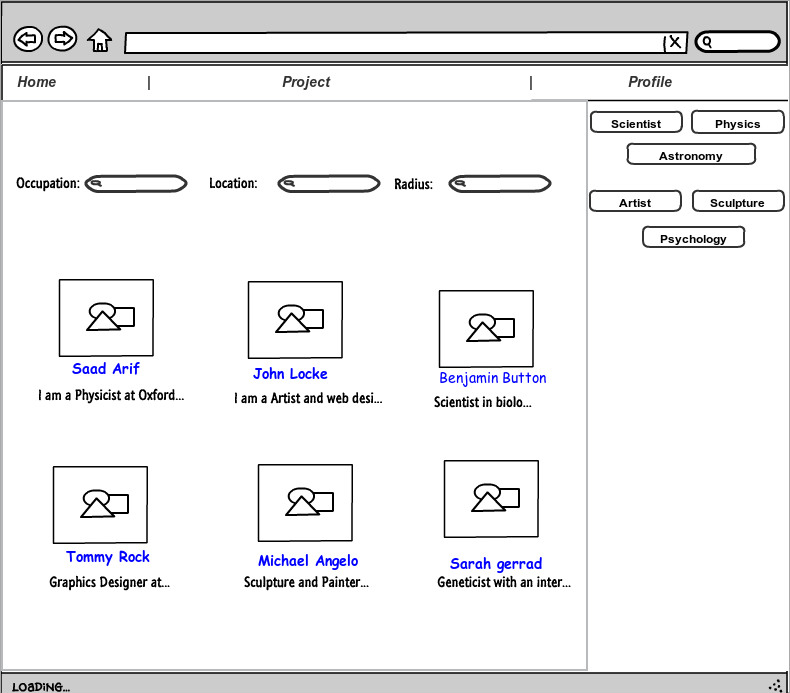
\includegraphics[width=\textwidth,height=10cm]{People.jpg}
\caption{Search Page}
\end{figure}
This interface design is above is for allowing users to search for collaborators. The search bars allow the users to search by area of work, location, by radius from a particular location, skills and interests.
Once the search is completed, a grid of member information will appear. Each member that matched the search criteria will have their profile picture, name and first few words of their biography shown. The far right hand side shows popular areas in which members have claimed they have expertise in.

\pagebreak
\subsubsection{Profile Page}
\begin{figure}[!ht]
\centering
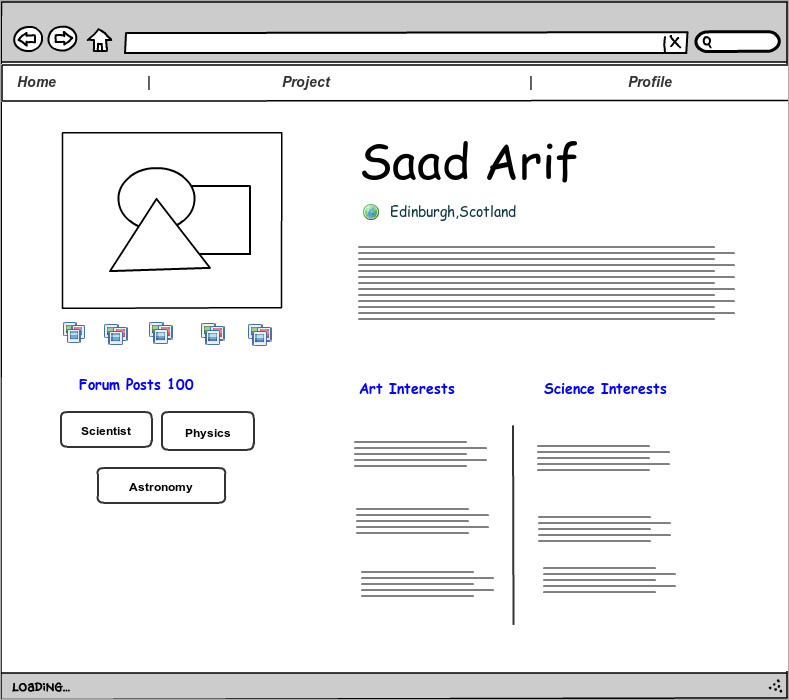
\includegraphics[width=\textwidth,height=10cm]{Profile.jpg}
\caption{Profile Page}
\end{figure}

The figure above shows the interface design for the second main requirement, the profile page. This shows how the profile page will look after the user has entered his/her details.


The profile contains useful information that other users are likely to be interested in. It includes location, small biography. Also specific part is dedicated to simply talk about artistic and scientific interests. This will allow for more freedom to say what interests the member regardless of occupation.

On the bottom left it also shows the areas in which the member has claimed to be an expert. Expertise area coupled with the artistic/scientific interest should give the user enough information to judge if the registered member is appropriate for collaboration.
\pagebreak

\subsubsection{Home Page}
\begin{figure}[!ht]
\centering
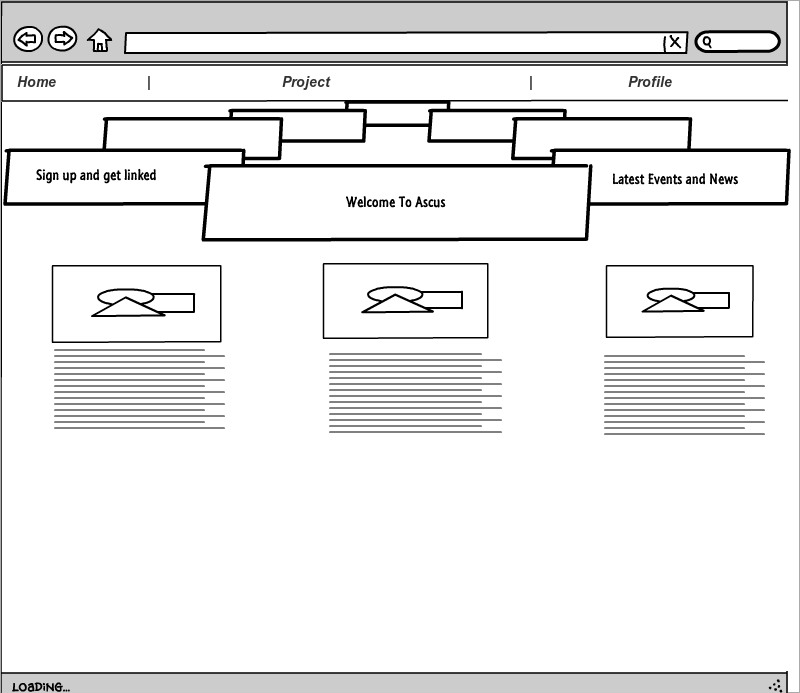
\includegraphics[width=\textwidth,height=10cm]{Homepage.jpg}
\caption{Home Page}
\end{figure}

The figure above shows the home page for the application. The purpose of this page is to introduce the user to the application as well as act as marketing tool to new users. This page should be aesthetically pleasing and contain information to hook the user in and use the application. The carousel acts as navigation tool as well as gives the user knowledge of what is available on this site quickly.
\pagebreak

\subsubsection{Log in}
\begin{figure}[!ht]
\centering
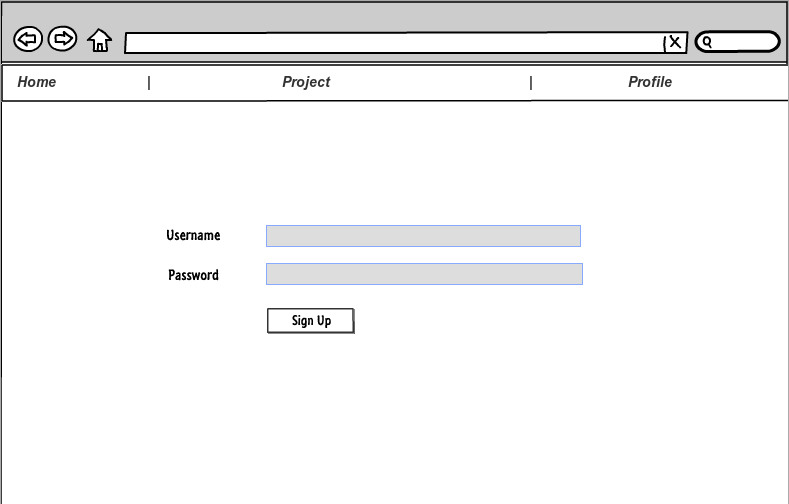
\includegraphics[width=\textwidth,height=10cm]{Log_in.jpg}
\caption{Log in Page}
\end{figure}

The above figure shows very standard log in page. Though not shown in the above figure, this page will also show error message when the user name and/or password is incorrect.
\subsection{Middleware}
The development in the middle tier consisted of a developing utility classes as well as implementing registration,login and logout functionality.

\subsubsection{Database Class}
PHP provides an an extension called PDO which defines an interface to allow users to access a database. It is generic and abstracts over the particular database being used. However using PDO requires boilerplate code on every access to the database. In order to simply the usage of PDO a Database class was created. It uses PDO internally and provides simpler interface which does not require boiler plate code. 
\subsubsection{Utility Classes}
Their were many utility classed created, their purpose was to provide convenience or simply hold functionality that was not appropriate in other classes.
\\
The following paragraphs detail the name and the purpose of the classes: 
\subparagraph{Input}
Input class allows convenient access to the POST and GET arrays. Input class allows the user to get a value without having to specify which array to get it from. It also has convenience methods to check if a value exists in the arrays or if the array its self is empty. 
\subparagraph{Session}
Allows access to the underlying SESSION variable. It allows the user to insert data, get back data, check if data exists in the SESSION variable. It also has a flash functionality. which allows a message to deleted after it is displayed. This is useful for messages that should be displayed only onces such as displaying a log in message when the user logs in.
\subparagraph{Hash}
Allows basic hashing functionality such as generating a hash and verifying if a value is the original value a hash. This is useful for securing passwords. It also generates unique numbers.
\subparagraph{Sanitize}
Provides basic method to sanitize value by converting any html elements in it into safe values. This is important when retrieving data that use has entered from the database.
\subparagraph{Redirect}
Convenience class for redirecting to a page by simply specifying its name. It also has special error pages built in as well, such that the user only needs to specify the error code and it will redirect to the page corresponding to the error code e.g. 404.
\subparagraph{Token}
Generates tokens and verifies tokens. Tokens help prevent cross site scripting attacks by ensuring a unique token is sent every time a user enters data.

\subsubsection{Registration, Login and Logout}
In order to implement member related functionality a member class was created. It allowed a member to register, login and logout. The registration details were taken from the registration page and then passed on to the member class. The member class would then insert the details into the database. An important thing to note is that, the member class uses the database class internally. Thus there is no need to sanitize the input as the database class does that automatically by using prepared statements. This means that one of the most common web application vulnerabilities called SQL injection are avoided.
\\
\\
The login and logout functionality was implemented using the session variable. When a user would log in the member class would store the member id, which is stored in the database, in the session. By doing this, it is now possible to simply check if the id is in the session, if so then the user is logged in. Furthermore now it is possible to stop users from accessing particular pages. To log the user out, the member id was deleted from the session.
\subsection{Back End}
In order for the database design to reflect the requirements, it is important to identify the separate entities with in the requirements. Two entities were identified, member who has registered and the members areas of expertise. The figure below shows the relation ship between these entities.

\begin{figure}[!ht]
\centering
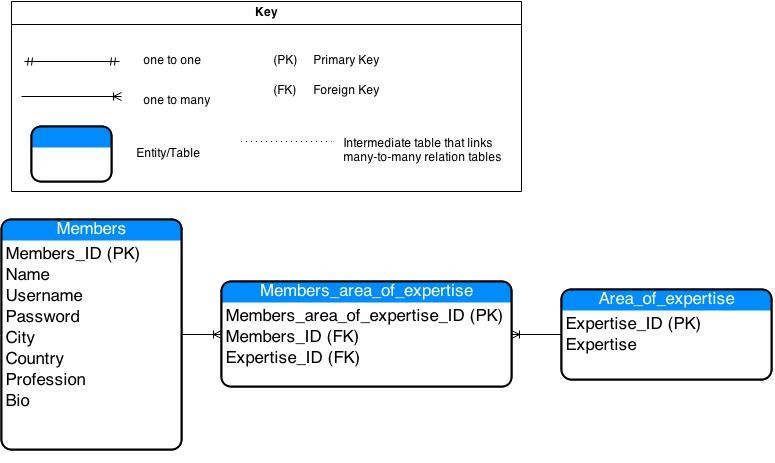
\includegraphics[width=\textwidth,height=10cm]{Iteration-1-ER-Diagram.jpg}
\caption{Initial ER-Diagram}
\end{figure}
\pagebreak
The initial database design stores login information as well as partial profile information in the members table. It makes sense to store that information in the members table as it is related to the member directly and it has 1 to 1 correspondence with a member i.e. every member has that information.

Every member has many expertise and a single expertise can be shared by many members. Thus we have a many-to-many relationship between member and expertise areas. In order for the many-to-many relationship to be implemented it must require an intermediate table. The members\_area\_of\_expertise table will act as link between the member and their expertise. It will use a surrogate primary key as well as a unique composite key. The composite key will be the members\_id and the expertise\_id combined. This way each member has a unique link to an expertise.
\section{Testing and Evaluation}
At this stage it was sufficient to manually test the system as only minimal functionality had been implemented. In the case of the evaluation, informal meeting were carried out with the client where feedback was given on the prototype and functionality implemented and a questionnaire was sent out.

Thorough the meetings was two main issue that was identified with the initial prototype. The profile page did not allow artists or scientist to display samples of their work. Samples of work would be an important indicator when searching for collaboration partners. It would be useful for artist to upload images of their work and scientist can give details of their research as well as links to the papers they have published.

Another issue with the initial prototype was lack of result information provided by the search. In the prototype only an image of the member,their name and a few words of them selves are provided in the search results. This forces users to go onto the members profile page to get further details and it slows down the process of searching for the user.

Furthermore issues were identified with the registration functionality. In its current form it did not stop potential users or bots from creating many accounts and creating fake profiles. The solution was to only allow members to login once they had verified their email address. By doing this even it forces the users to put more effort into making an account as they would have to provide a legitimate email address.

The questionnaire was used to evaluate and understand the two most important pages of the web application, the profile and the search page. The figures below highlight the results for three questions in the questionnaire.

\begin{figure}[!ht]
\centering
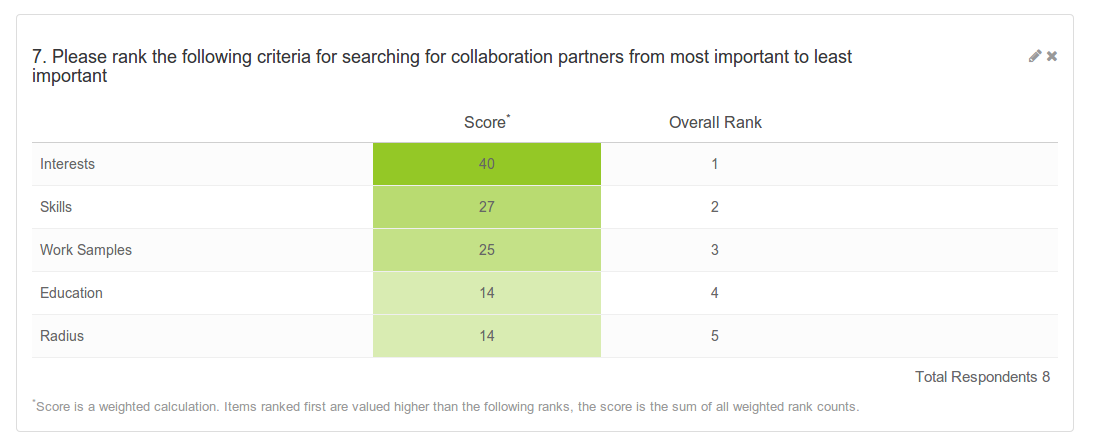
\includegraphics[width=\textwidth,height=6cm]{questionnaire-iteration-1-q7.png}
\caption{Question 7 of the questionnaire}
\end{figure}
\begin{figure}[!ht]
\centering
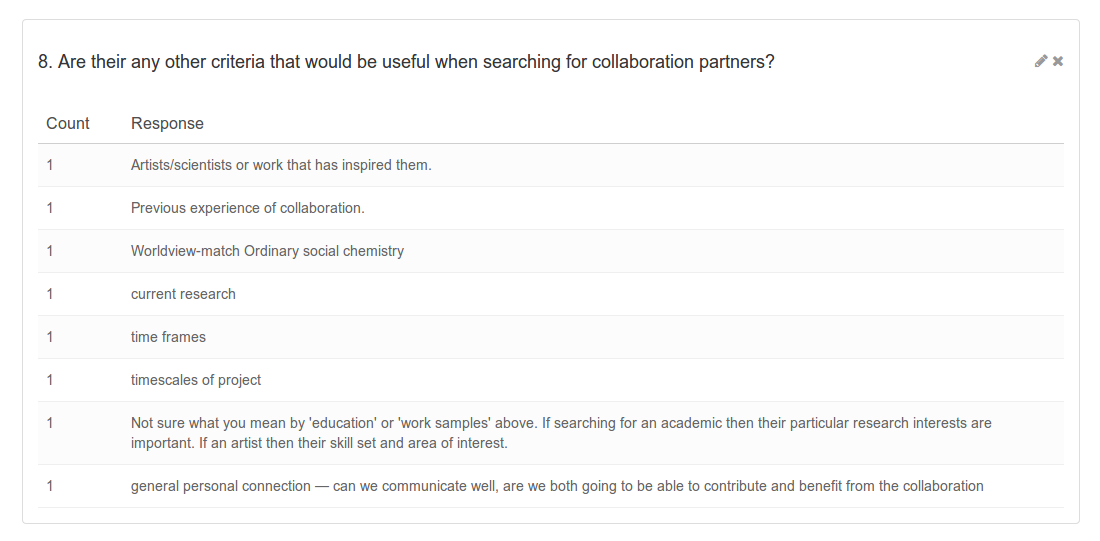
\includegraphics[width=\textwidth,height=6cm]{questionnaire-iteration-1-q8.png}
\caption{Question 8 of the questionnaire}
\end{figure}
\begin{figure}[!ht]
\centering
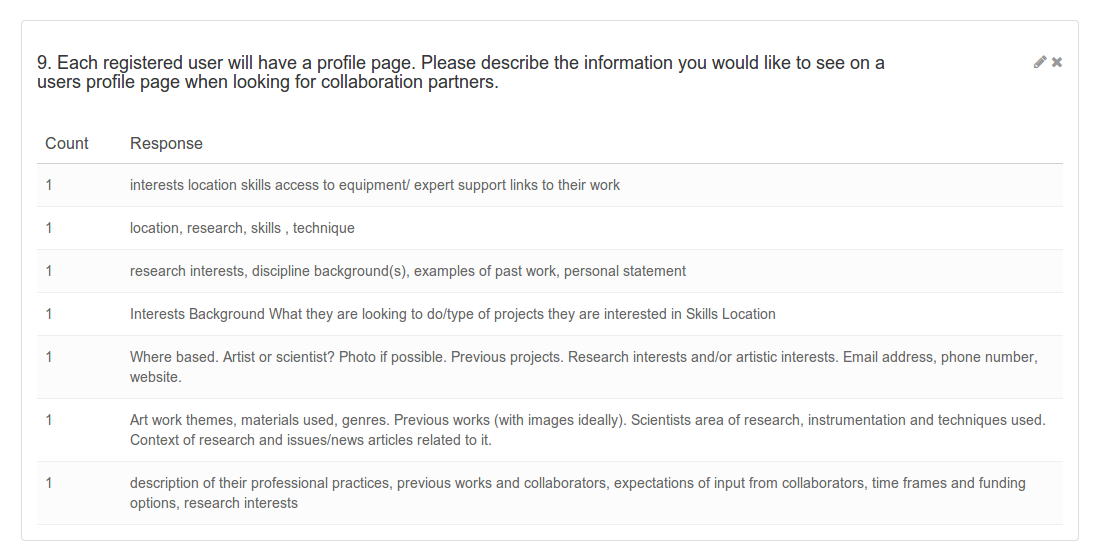
\includegraphics[width=\textwidth,height=6cm]{questionnaire-iteration-1-q9.png}
\caption{Question 9 of the questionnaire}
\end{figure}
\newpage
Figure 5.6 shows that the most important search criteria to users were the interests and expertise criteria, while the least important was radius. From the results it makes sense to remove radius criteria as it is the least valued and the removal will simplify the search page. Furthermore the original idea for search by radius was primary to search within a city user was living in. However in order to implement this functionality, the post code of user would be required, in order to get a accurate results. Since this information is very personal to the user and since this information is unlikely to be obtained in majority of cases, it makes this feature obsolete.

Figure 5.7 shows a new search criteria that was missed from previous meetings, searching by availability of the user. This would help narrow the search for a potential collaborator as people are only available or willing to collaborate for certain periods of time. This would complement the project section of the web application, as users would be able to add the time frame of a project.

Lastly figure 5.8 confirms the direction that the information provide on the profile page as initially decided was generally correct. Though there is specific information that users are looking for such as scientific techniques used, profession practices etc, they are too specific to have their own section on the profile page. In majority of cases this information would not be useful to users. Thus a preferable solution is to allow the user to put information as they see fit. This means that a wide variety of information can be put on the profile page without restricting the user.
\chapter{Second Iteration}
This chapter describes the development of the project in the second iteration. The second iteration involved implementing the prototype created in the previous iteration as well as incorporating the feedback received.
\section{Requirements}
The requirements did not change from the previous iteration, as through informal meetings it was decided the requirements were sensible for the time available for this project.
\section{Design}
This section details the expansion of prototype from a concept prototype to a work in progress web application. This section also details how the user interface was improved based on the feedback in the previous iteration as well as what extra functionality was implemented.
\subsection{Front End}
\pagebreak

\subsubsection{Responsive Design}
Responsive design refers to a design of a website or web application which provides the same viewing experience across a wide range of devices. The primary feature of responsive design is the flexibility of the layout. The layout can increase in size on a larger screen as well as shrink and fit optimally on a smaller screen.

In order to achieve this requirement the Bootstrap framework was used. Bootstrap provides css classes and javascript functionality to achieve responsive design. By using the provided css classes the web page will automatically scale into the appropriate size. However Bootstrap is very generic and requires customization in order to get the appropriate design . Thus even by using bootstrap, some effort must still be put into making the web pages responsive.

This prototype was built using bootstrap however there was not a large focus in making it responsive in this iteration.It was anticipated that many changes would occur before this prototype would become fit of release and thus it would quicker to make the web page responsive once the final design was set.

\subsubsection{Search Page}
\begin{figure}[!ht]
\centering
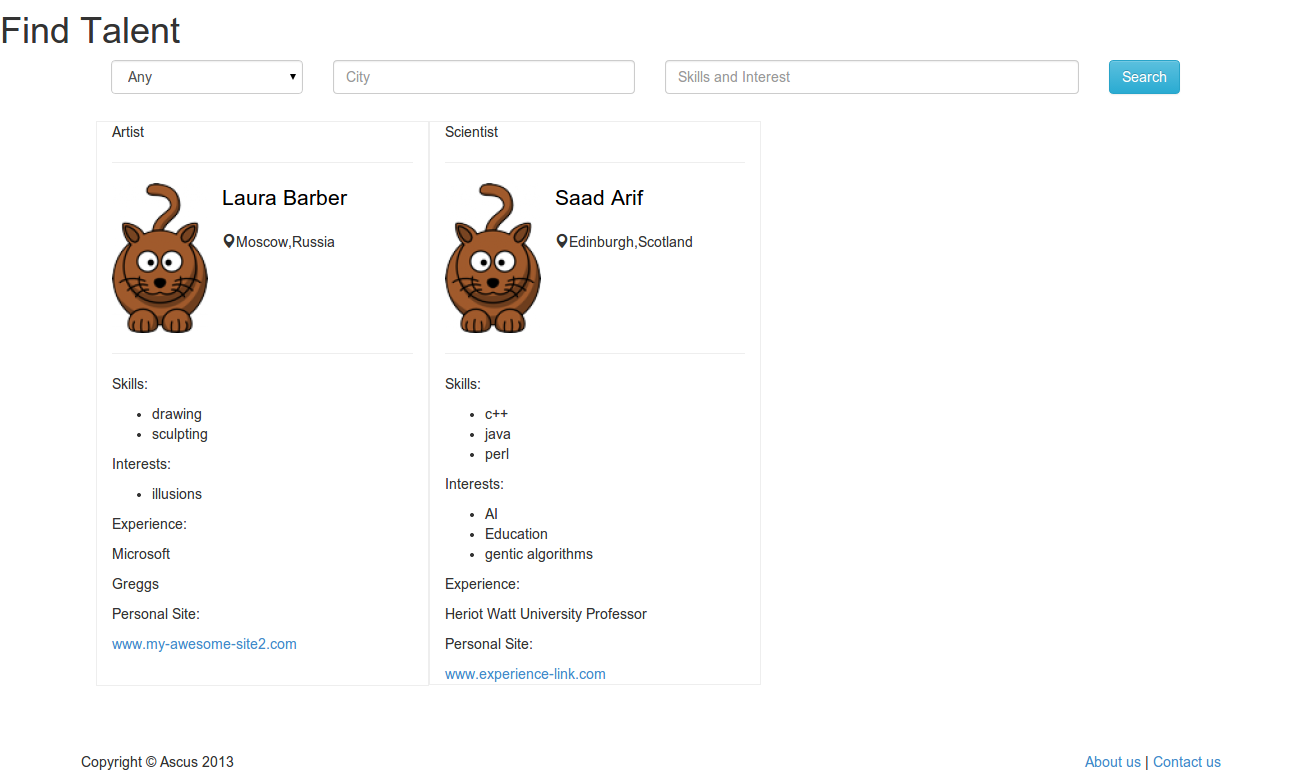
\includegraphics[width=\textwidth,height=10cm]{search-second-iteration.png}
\caption{Search Page}
\end{figure}
Their were several changes were made to the search page based on the feed back received. The major change was to return extra information when the search had finished. After the user completes a search a ``mini profile" is returned of those members that matched the search criteria. The mini profile details the name,location, skills, interests, experience and a link to their personal site. The mini profile does not show all the users skills, interests or experiences but only the first three. This is done in order to simplify the search results and allow the user to quickly discern appropriate candidates for collaboration. If the user requires more information about a particular member they can click on the members name and it will take them to the members profile. 

The search criteria was also simplified to four options and three ways to input data. The user can search for collaboration by their profession; artist, scientist or either. They can search by the city in which the member lives in and they can search by skills or interests the members have. The skills and interests input field was combined into one as to simply the options available to the user. The search by radius criteria was removed based on discussion in the previous iteration, testing and evaluation section.
\pagebreak

\subsubsection{Profile Page}
\begin{figure}[!ht]
\centering
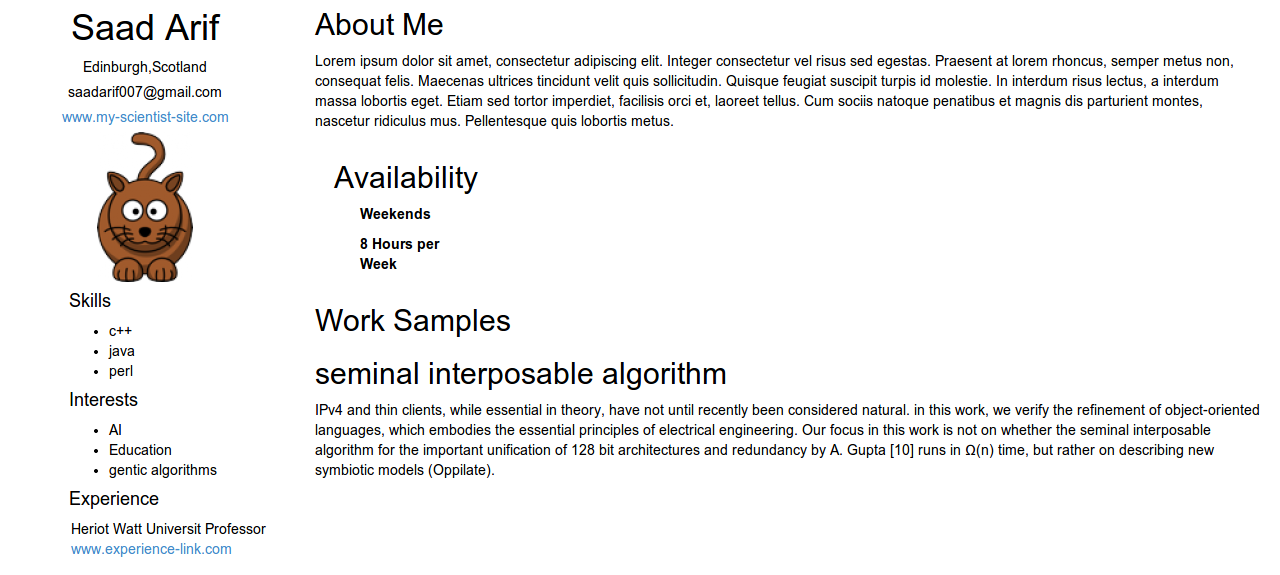
\includegraphics[width=\textwidth,height=10cm,keepaspectratio]{profile-second-iteration.png}
\caption{Profile Page}
\end{figure}
Several aesthetic changes were made to the implementation of the profile page that were not present in the prototype. However two major changes were made to the original prototype, these were the added display of how available a member was for collaboration and the display of work samples of the member. The availability section shows a rough estimate on how long the members are willing to work on collaborating per week. In the second iteration only scientist could add work samples, the work sample display would show title and description of their work. They were encouraged to add links to sites which could give further information on their work.

In order to keep the profile page short, the original interest section was changed into small key words, similar to how the skills section is. This meant all the information needed by a user could fit onto their screen at one time. However originally the interest section was quite large and allowed users to essentially enter large amounts of information. In order compromise for the shrinking of the interest section, the members were allowed to enter a link to their personal site. This would allow users to get more information on the members if they needed as well as getting a good summary from their profile page.
\pagebreak

\subsubsection{Edit Profile Page}
\begin{figure}[!ht]
\centering
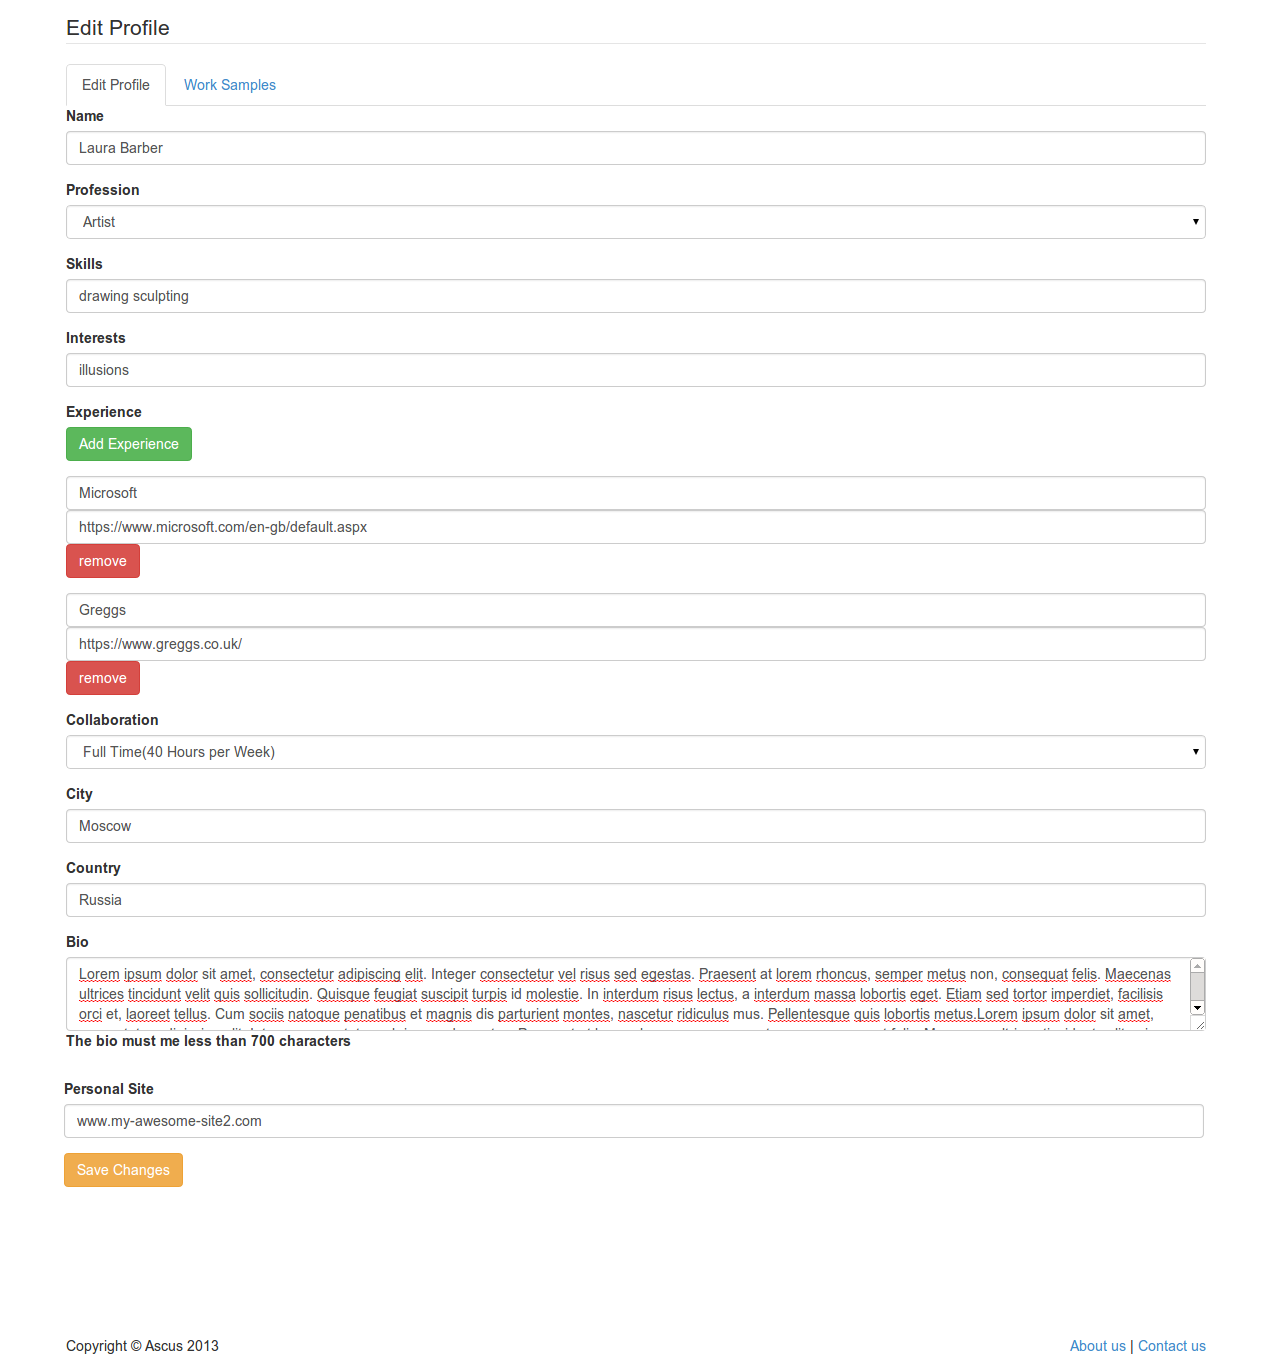
\includegraphics[width=\textwidth,height=15cm,keepaspectratio]{edit-profile-second-iteration.png}
\caption{Edit Profile Page}
\end{figure}
The Edit profile page allows a member to enter information that will be displayed on their profile. This page was not originally in the prototype as it was assumed to be a very simply input form. However it does incorporate the collaboration availability field that was added due to the result of the questionnaire in the previous iteration. It allows the user to enter one of the follow options; Weekends(8 Hours a week),
Part Time(20 Hours per Week),Full Time(40 Hours per Week), Everyday(60 Hours per Week). This allows the members to enter a variety options to convey their availability and time they are willing to put in a collaboration project. It should be noted their is front end validation being used on the bio input field and is explained in the validation section of the front end section.
\pagebreak

\subsubsection{Show Work Sample Page}
\begin{figure}[!ht]
\centering
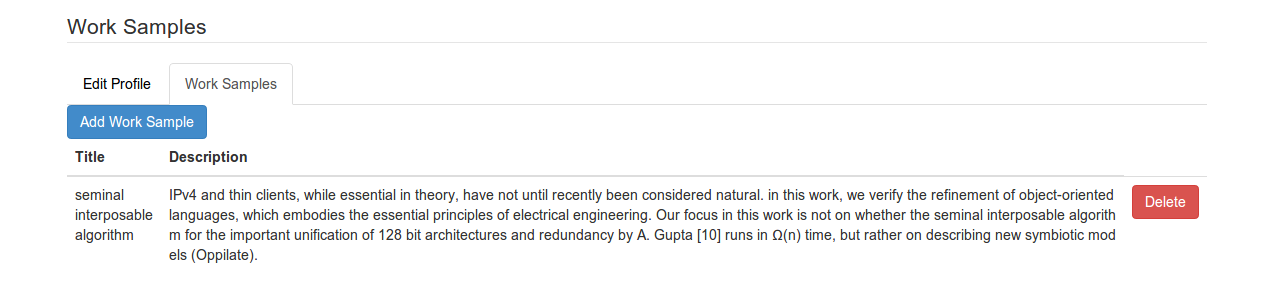
\includegraphics[width=\textwidth,height=5cm]{show-worksample-second-iteration.png}
\caption{Show Work Sample Page}
\end{figure}	
This page allows members to manage their work samples. They can add more work samples or delete ones they have already added. In this iteration the show work samples page only displays the work samples for scientists.
\\

\subsubsection{Add Work Sample Page}
\begin{figure}[!ht]
\centering
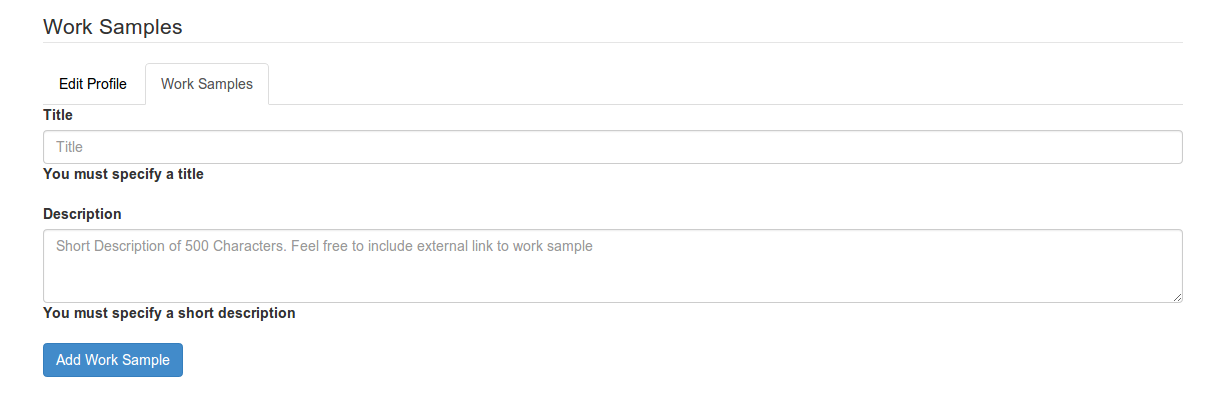
\includegraphics[width=\textwidth,height=10cm,keepaspectratio]{add-worksample-second-iteration.png}
\caption{Add Work Sample Page}
\end{figure}

This page allows the members to add work samples. It performs basic front end validation, to ensure a title is entered and description of is kept at a reasonable length.
\pagebreak

\subsubsection{Registration Page}
\begin{figure}[!ht]
\centering
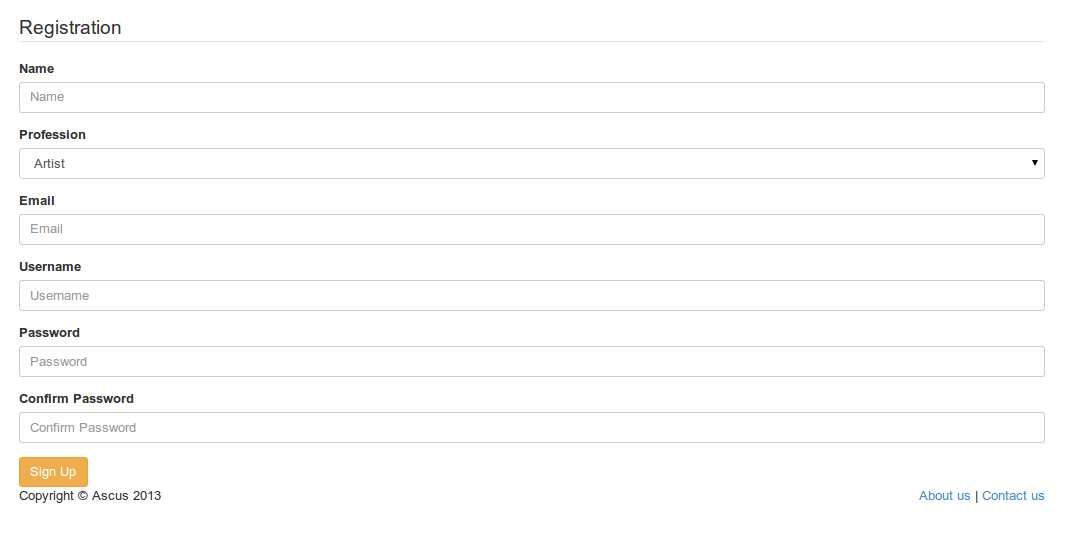
\includegraphics[width=\textwidth,height=10cm,keepaspectratio]{registration-second-iteration.png}
\caption{Registration Page}
\end{figure}

The is page is a standard registration page, which allows the user to become a member. Originally the registration page was to be kept as simple as possible. This was done with the thought, that users are likely to sign up if signing up is very quick and did not require any significant information. However simplicity and quick registration were in contention with the email verification feature discussed in the previous iteration's feedback. In order to implement email verification the registration required a valid email address from the users. This slowed down the registration process as users needed to enter an extra field of information and more importantly forced the user to give their email address. For many users having to provide their email address may turn the away from the web application however it was decided this was an acceptable risk.
\pagebreak
\subsubsection{Front End Validation}
Validation is carried out on data given by user to ensure reasonable data is entered. Front end validation involves carrying out validation on the clients machine before the data gets sent to server. Front end validation is useful as it saves the users time because any mistakes can be corrected before the data is sent to the server and thus the page does not need to be refreshed. If the page is refreshed all previously entered data is lost and has to be re-entered.

In order to carry out validation a jquery library was used called jquery validation. This saved time as the author did not have to implement it himself and it was already tested against bugs. The jquery validation many common types of validation such making a field mandatory, only allowing field to include letters etc. 

The front end validation involved basic sanity check such as making sure no numbers have been entered into name field, confirm password matched to the original password entered etc. However validation on the bio field on the edit profile and description field on the add work sample page was carried out. This was done in order ensure that the bio and description of work samples were kept to a minimum. By doing so it forces the writer to make it simpler and easier to understand. This was done mainly from perspective of artist trying to understand a scientists work.

The jquery validation library did not provide all the functionality required , it didn’t provide a way to ensure that the email entered was unique. This functionality was needed to ensure that users did not enter someone else’s email and to avoid account spamming( a single user creating lots of accounts). Ajax was used to implement this functionality. Ajax allows requests to be made to the server in the background, from clients perspective the page does not refresh. Using ajax allows to keep the appearance as if all validation occurred on the client side.


\subsection{Middleware}
In the second iteration the edit profile, add work sample functionality was implemented. Furthermore server side validation was also implemented in order to complement the front end validation.

\pagebreak

\subsubsection{Middleware Validation}
While front end validation provides validation as well as user convenience it can be easily circumvented. Front end validation relies jquery running on the clients machine. However the user can easily stop this by prevent jquery to run by choosing the appropriate options available in their web browser. In order to stop such a security breach, server side validation was also implemented.

Figure 6.7 shows the high level design of the validators using a class diagram.All validators inherit from an abstract class called Validator. This implements the basic functionality required by all validators. All validators must have validate method, which takes in a value to be validated and field name so the error message returned is customized. Several validators require functionality in order to function, such as the UniqueValidator which connects to the database to check if a value is unique.

The ValidatorManager takes in validators through the add validator method and simply runs each one on the value specified. It also puts all the validator error messages in the error variable.

The following code shows a typical uses of the validator:
\begin{lstlisting}
	$validatorManager = new ValidatorManager();	
        $validatorManager->addValidator(new RequiredValidator())
                ->addValidator(new EmailValidator())
                ->addValidator(new UniqueValidator('email'));
        $validatorManager->validate(Input::get('email'), "Email");
\end{lstlisting}

\begin{sidewaysfigure}[htbp]
\centering
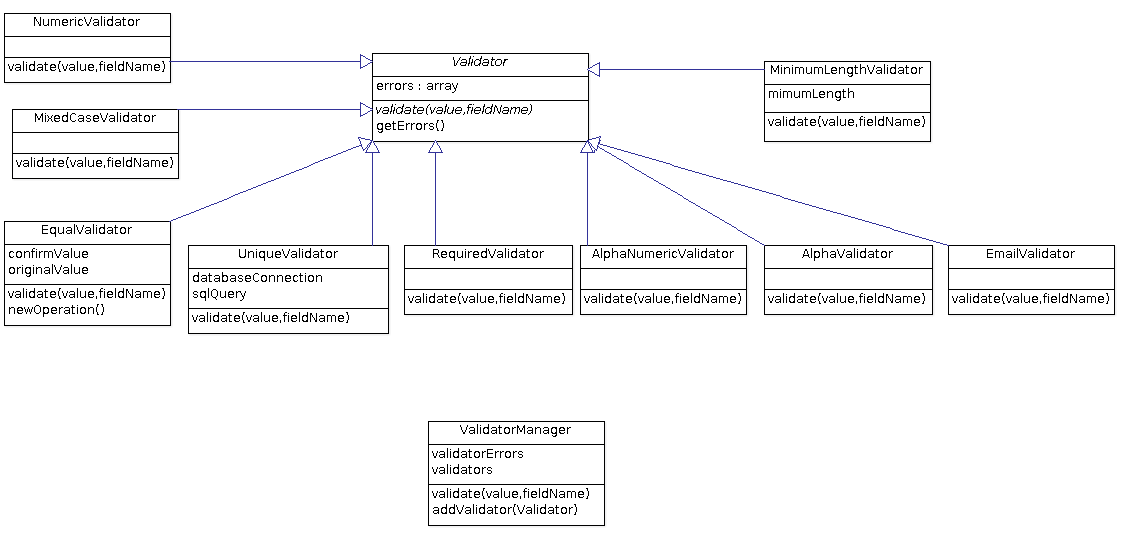
\includegraphics[width=\textwidth,height=11cm]{validator-class-diagram}
\caption{Validators Class Diagram}
\end{sidewaysfigure}

\pagebreak
\subsubsection{Add Work Samples and Show Work Samples}
In order to manage work sample related functionality a work sample class was created, called WorkSample. The WorkSample class creates an abstraction over database table related to work samples. The WorkSample class provides three methods, addWorkSample and delete and findByMemberId. To display the work samples the findByMemberId method is used in conjunction with the Member class to the get the id of the member and then use that id to get all work samples of the member.

\subsubsection{Email Verification}
This functionality involved sending an email to the user once they had registered. The email would contain link to activate verify their email address. Furthermore the user must not have access to their profile before the email address is verified.

In order to implement this feature a library called PHPMailer was used. PHPMailer simplified the process of sending an email and also allowed embedded html for more customization.

In order to link the activation of a particular email address to a particular user, a unique identifier was added to the link. When the user clicks the link the unique identifier is passed through the url to the confirmation page. The confirmation page then updates the database and redirects the user to the home page and shows an appropriate message, which signals the email has been verified.

\subsubsection{Edit Profile}
The edit profile functionality was implemented using variety of classes. The majority of information is stored in the members table and thus the Member class is used for that purpose. The Member class provides an edit member function which adds the name,profession, collaboration availability, city, country, bio and link to the personal site to the Members table. The addition of experience, interest and skills is handled by the Experience, Interest and Expertise class respectively. Internally these classes do not overwrite the old data entered, they simply add to their respective tables using the ``REPLACE INTO" query.

Edit profile page fields are filled in with the information that is already stored in the database. However database has to be updated based on the changes made in the fronted but in order to do this, the difference between what is in the database and what has been given by the user has to be calculated. 
\pagebreak

An example of this would be a member had an interest "illusion" and deleted and added a new interest "drawing". This change of deletion of old values and insertion of new values has to reflected in the database.

This problem has two solutions, either calculate the difference, if their is a difference the apply the difference, this may mean deleting some elements and inserting new elements at the same time. The other solutions is to simply delete all old data and then insert the new data. The latter of the two choices was chosen, even though conceptually the latter decision may be inefficient, its simpler to implement. For the small amount of values entered their is no significant performance difference.
\pagebreak
\subsection{Back End}
Several changes were made to the back end database in order to implement the new functionality. Interest, Experiences,Work\_Samples tables were added to hold information on interests, experiences and work samples added by the members.

The Email, Confirmation\_Key and Status fields were added to the members table in order to implement the email verification functionality. The Confirmation\_Key field would hold the unique identifier sent to the user. The Status field was used to hold 0 for if the email had not been verified and 1 if it had.

It should be pointed out that the link between expertise and members uses an intermediary table while the interests,experiences does not. It is an oversight in the design of the database and premature optimization, as the members were expected to share many expertise however it was felt members were unlikely to share interests or experiences. The correct decision would have to been to make it a 1 to many relation as this would have simplified the interaction with relation through the middleware. Overall it is minor oversight and fixing it is of low priority.
\pagebreak			
\begin{figure}[!ht]
\centering
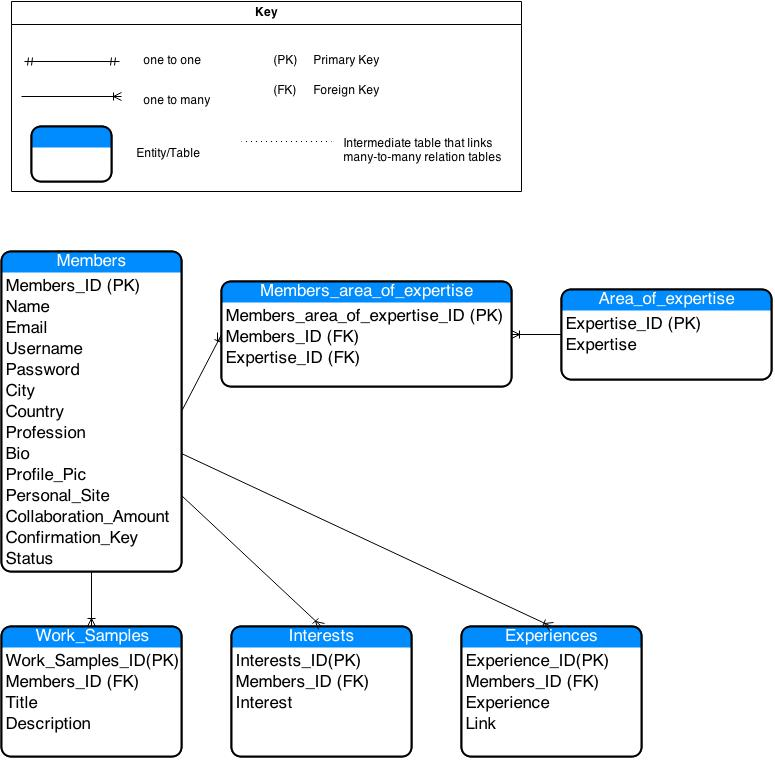
\includegraphics[width=\textwidth,height=15cm]{second-iteration-er-diagram.jpg}
\caption{Second Iteration ER Diagram}
\end{figure}
\section{Testing and Evaluation}
As this was a work in progress prototype, some major features were available for testing and evaluation. During this iteration feedback on the user interface and the implemented functionality was received through informal meetings. The overall feedback received was positive, However users wished add to their profile, extra types of work they were willing to do. Specifically they were willing to do paid and or volunteer work.

The testing was split into two parts, the first part consisted of features that could be tested easily using unit testing i.e. the validators. The second part consisted of features that were tested manually.

The validators implemented were tested using unit tests because they were decoupled from other functionality and consisted of a small enough unit that could be tested easily. In this iteration all the unit tests passed.

The manual testing involved testing by carrying out tasks or using feature that was implemented.
The following table shows the result of the manual testing.

\begin{center}
	\begin{table}[!ht]
    \begin{tabular}[ht]{| p{5cm} | p{5cm} | l |}
    \hline
    Test Action & Expected Results & Actual Results \\ 
    \hline
    Register as a user & the user is added to the database and an email verification link is sent to the users email address & as expected \\
    \hline
    Accessing the profile page without verifying their email address & the user will be redirected to the home page with an appropriate message & as expected \\
    \hline
    Verify email address by clicking the link provided in the email & the user is redirected to the homepage and is given an appropriate message. The database is updated to reflect the user has verified their email & as expected \\
    \hline
    Edit profile details & The database reflects the changed details. The edit profile page is refreshed and shows the new details. The profile page reflects the changed made & as expected \\
    \hline
    Add a work sample & the work sample sample is added to the database. The work sample page and the profile page show the new work sample. & as expected \\ 
    \hline
    Delete a work sample & the work sample is deleted from the database. The work sample page and the profile do not show the any work samples. & as expected \\
    \hline
    \end{tabular}
    \caption{Testing Results}
\label{tab:xyz}
    \end{table}
    \end{center}

\chapter{Third Iteration}
This chapter describes the development of the final release. This release builds on the feedback received from the previous iteration. Any changes after this iteration will only consist of bug fixes and no new features will be added.
\section{Design}
During the final design stages of the application there were many changes made in order to make it suitable as a final release.  The middleware and back end development involved adding the search functionality, allowing artists to add work samples to their profiles and allow both artists and scientists to upload a profile pictures.
\subsection{Front End}
This section will explain developed in the front end tier during this iteration. The front end development involved designing the finished user interface and increasing the usability by adding simple features such as helpful error messages. It also involved ensuring that the application was responsive and displayed correctly on the specified devices.
\subsubsection{Responsive Design}
Responsive design was achieved using functionality provided by the bootstrap framework. The most important css classes were ``col-md" and col-sm". The col-md class works for medium sized devices such as computer screens and sm works for small devices such as tablets and some mobile phones. By using these classes, the layout was split into flexible columns – resizing when the screen size changed. See the appendix for images of the user interface on different screen sizes. It should be noted even though Bootstraps documentation states the col-xs class should be used for mobile devices, in the case of this project it sufficed to use the col-sm classes. Thus there is no guarantee that the web application will look appropriate on other devices which are not stated in the requirements.

\subsubsection{Work Type - Edit profile}
In the previous iterations feedback, many users asked for the ability to add particular type of work they are willing to do. The conclusion was to include three types of options volunteer work, paid work and no collaboration. In this case collaboration work comes under volunteer work. While collaboration work implies working as peers Volunteer does not and covers a larger domain. The following figure shows the user interface for the options.

\begin{figure}[!ht]
\centering
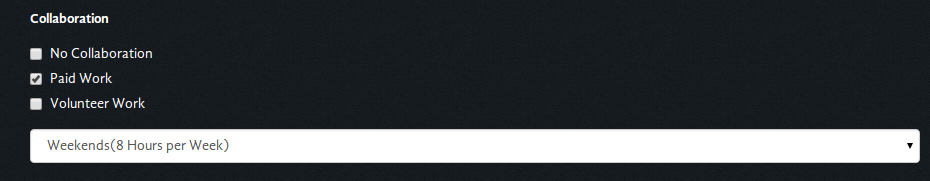
\includegraphics[width=\textwidth,height=3cm]{third-iteration-collaboration-availability.png}
\caption{Second Iteration ER Diagram}
\end{figure}

Checkboxes are used so multiple options can be chosen at once.
\subsection{Middleware}
\subsection{Back End}
\section{Testing and Evaluation}

\chapter{Risks Assessment}
 	This section will give an an overview of the potential risks to project development.
\begin{center}
	\begin{table}[!ht]
    \begin{tabular}[ht]{| l | l | l | p{5cm} |}
    \hline
    Risk & Probability & Severity & Mitigation Strategy \\ 
    \hline
    Browser compatibility issues & High & Moderate & Constantly test browser compatibility through out the development cycle. Leverage automatic test frameworks in order to supplement manual testing.\\ \hline
    Fall behind on plan & Moderate & Moderate & Give small leeway time for each part of the application. If significantly behind schedule then only complete vital parts of the application.  \\ \hline
    Person of interest is unavailable & Moderate & Moderate &  Another client is kept up to date with the main development of the application.\\ 
    \hline
Users find the system unusable & Moderate & High & Follow user centred design approach. Maintain regular meetings with the client. User testing must be carried out extensively and feedback should be integrated into the next iteration. \\ 
    \hline
    Low quality feedback & Low & Moderate & Pilot all methods used to gain user feedback. If low quality feedback is given reassess previous methods for weaknesses and integrated any finding. \\ 
    \hline
    
    \end{tabular}
    \caption{Risk Assessment}
\label{tab:xyz}
    \end{table}
    \end{center}


\chapter{Project Plan}
A high level plan below describes the key tasks to be achieved.
\begin{center}
	\begin{table}[!ht]
    \begin{tabular}[ht]{| l | l | p{11cm} |}
    \hline
    Due Date & Version & Task \\ 
    \hline
    15/10/2013 & R1 & Gather initial requirements.\\ 
    \hline
    01/11/2013 & N/A & Conduct Literature review and research into relevant 												  technologies \\ 
    \hline
    22/11/2013 & Final & Hand in final version of the first deliverable \\ 
    \hline
    03/12/2013 & R2 & Create Questionnaire to gather further requirements. Pilot the 										questionnaire and improve it if needed.\\ 
    \hline
    31/12/2013 & WD1 & Create Website design prototype.\\
    \hline
    31/12/2013 & DD1 & Create initial database design and implementation.\\
    \hline
    31/12/2013 & IMP1 & Create an initial implementation of high priority requirements\\
    \hline
    10/01/2014 & N/A & Gather feedback on initial prototype and implementations. Improve 	                  				   the current system according to feedback.\\
    \hline
     17/01/2014 & WD2 & Create website design prototype for high and medium priority 										  requirements.\\
    \hline
    27/01/2014 & DD2 & Update database design in order to facilitate high and medium 		 								 priorities.\\
    \hline
    07/02/2014 & IMP2 & Implement medium priority requirements and integrate with previous requirements.		\\
    \hline
    17/02/2014 & N/A & Gather feedback and improve system based on feedback.\\
    \hline
    27/02/2014 & Final & Create final website design prototype for high,medium and low priority 			 			 requirements.\\
    \hline
    07/03/2014 & Final & Final update to database design in order to facilitate high,medium and low		 		             priorities.\\
    \hline
    17/03/2014 & Final & Implement low priority requirements and integrate with previous requirements.\\
    \hline
    01/04/2014 & Final & Test the systems, fix any bugs and release the system.\\
    \hline
    \end{tabular}
    \caption{Project Plan}
\label{tab:test}
    \end{table}
    \end{center}

\printbibliography
\end{document}
